\begin{figure}[h]
    \centering
    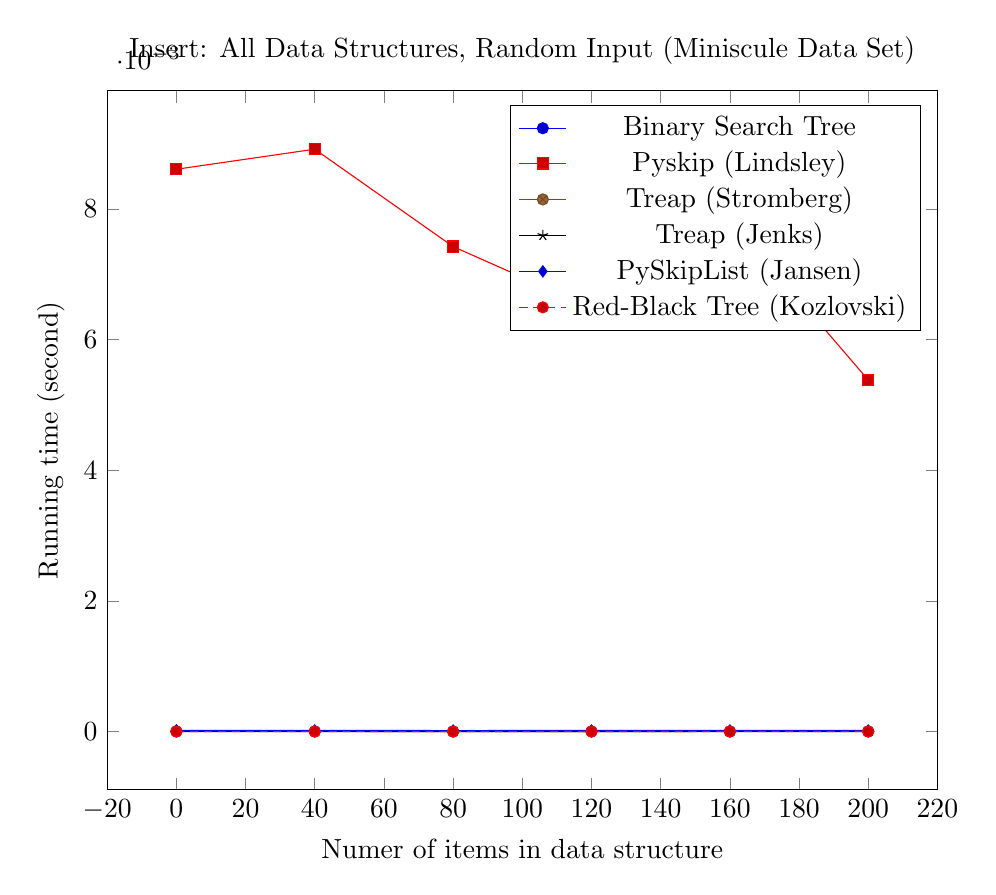
\begin{tikzpicture}
        \begin{axis}[
            xlabel={Numer of items in data structure},
            ylabel={Running time (second)},
            title={Insert: All Data Structures, Random Input (Miniscule Data Set)},
            width=\textwidth
        ]
		\addplot coordinates {
			(0, 5.360920994146312e-06)
			(40, 5.300685926812321e-06)
			(80, 4.999510590142364e-06)
			(120, 5.903036600329869e-06)
			(160, 5.601861263571095e-06)
			(200, 5.752448931950483e-06)
		};
		\addplot coordinates {
			(0, 0.008605784072342271)
			(40, 0.008912802210626935)
			(80, 0.007422827584649116)
			(120, 0.006483190651517567)
			(160, 0.00784778598480571)
			(200, 0.005382214090488091)
		};
		\addplot coordinates {
			(0, 7.679971087171112e-06)
			(40, 5.360920994146312e-06)
			(80, 4.306807315579419e-06)
			(120, 4.427277450247402e-06)
			(160, 5.180215792144338e-06)
			(200, 5.270568393189734e-06)
		};
		\addplot coordinates {
			(0, 2.6202254296947556e-06)
			(40, 2.4696377614041864e-06)
			(80, 2.2286974919794033e-06)
			(120, 2.288932559313395e-06)
			(160, 2.0781098236000163e-06)
			(200, 2.620225429783574e-06)
		};
		\addplot coordinates {
			(0, 2.153403657780828e-05)
			(40, 1.9726984557255633e-05)
			(80, 1.843193060917514e-05)
			(120, 1.9275221552117473e-05)
			(160, 1.9486044287830852e-05)
			(200, 1.903428128269269e-05)
		};
		\addplot coordinates {
			(0, 2.710578030740152e-06)
			(40, 2.921400766542348e-06)
			(80, 3.162341035878313e-06)
			(120, 3.463516372637088e-06)
			(160, 3.493633906348492e-06)
			(200, 3.463516372637088e-06)
		};
        \legend{Binary Search Tree, Pyskip (Lindsley), Treap (Stromberg), Treap (Jenks), PySkipList (Jansen), Red-Black Tree (Kozlovski)}
        \end{axis}
    \end{tikzpicture}
    \caption{Average of 10 operations, benchmarked every 40, starting at 0.}
\end{figure}